\chapter{Introduction to Cloud}
In this section we will see the roots of cloud computing, which is a weird brew of different concepts: hardware virtualization, internet technologies, distributed systems and system management.

We'll go rapidly through the various concepts needed.
\section{Distributed Systems}
We have talked extensively about Distributed systems previously, just as a refresher, a distributed system is an heterogeneous set of $N$ autonomous processors (sites), $n$ administrators, $n$ operating systems, $n$ data/control flows.

\section{SOA}
A SOA is a Service Oriented Architecture, it's an open standard for software integrazion and uses a standardized web service software stack.

A Service Oriented Architecture implements the concepts of distributed system and computing providing a loosely-coupled, standard and protocol independent system. SOA used a protocol called SOAP that was very complex to use but very descriptive. Service Oriented Architectures aren't all that used anymore in web development because it's much easier to setup REST applications.

Cloud applications are developed as service compositions at different layers.

\section{Computing models}
There are many different computing models, we'll see a couple of them in the following:
\begin{itemize}
    \item Cluster computing: computers are interconnected through an high performance network and basically form a unique entity.
    \item Network computing: cluster computing extended to WAN.
    \item Meta computing: very old technique for distributed computing.
    \item Grid computing: Coordinated resource sharing and problem solving in a dynamic, multi institutional virtual organizations.

    This model relies on Web Service standard protocols.
    \item Utility computing: On demand delivery of infrastructure, applications, and business processes in a security rich, shared, scalable, and standard-based computer environment over the internet for a fee.
    \item Autonomic computing: autonomic systems with self management that provide adaptation mechanisms and reduce user involvement.
\end{itemize}

\section{Cloud computing}
Cloud computing is a mashup of some of the previous computing models, in particular autonomic and distributed systems.

The idea of cloud computing is to provide IT as a service. Storage, data processing and additional IT services distributed by external providers, applications are computing utilities and users have no need to know how they work beneath. The user pays as he goes depending on the type of service required.

As for distributed systems there are many different definitions for cloud computing, the more interesting one is the NIST definition, which follows:
\begin{center}
    \textit{Cloud computing is a model for enabling ubiquitous, convenient, on-demand network access to a shared pool of configurable computing resources that can be rapidly provisioned and released with minimal management effort or service provider interaction. This cloud model is composed of five essential characteristics, three service models, and four deployment models.}
\end{center}
We'll now go through the essential characteristics of cloud computing, if a cloud architecture doesn't implement all of them the architecture will perform bad and won't be used by many people as a result.
\begin{itemize}
    \item On demand, self-service

    A client can procure resources, server time and network storage on demand.
    \item Broad network access

    Accessing the cloud platform should be easy and should be supported via standard web protocols on any device.
    \item Rapid elasticity

    The network should be able to scale out, in and down\footnote{
        The difference between scaling in and scaling down is that scaling in involves adding resources to handle increased demand, while scaling down involves reducing resources as demand decreases.
    } automatically depending on the load. There should be minimal-to-none resource waste.
    \item Measured service

    Resource usage is monitored, controlled, and logged providing transparency to cloud providers and customers.
    \item Resource pooling
\end{itemize}
Some additional characteristics are the following
\begin{itemize}
    \item Lower costs
    \item Ease of use
    \item Quality of Service
    \item Reliability
    \item Outsourced IT management
\end{itemize}
A fundamental aspect of cloud computing is Multi-tenancy which means that a aingle software instance is shared by different enterprises/clients (tenants). Data, via virtualization, is isolated but we have no physical isolation.

The pros of multi-tenancy are that the cloud provider pays less for hardware and he can provide dynamic access to shared resources.

The cons are that users might access data of other users and data backup and data restore are more difficult.

\section{Infrastructure as a Service}
Users manage the whole machine, they have virtualized hardware resources associated to them and can install basically anything on the machines as if they had a box next to them. The user has a limited control of network components.

Companies provide different servers with different operating systems and an ad hoc software stack.

The advantages of IaaS are:
\begin{itemize}
    \item Pay per use
    \item Modular scalability
    \item Sercurity
    \item Reliability
    \item APIs
\end{itemize}
An example can be having a virtual machine with Linux and using it via the network to handle an heavy compilation process.

\section{Platform as a Service}
Users install and create applications developed using programming languages, libraries, services and tools supported by the provider.

An example of PaaS is ReplIT which is a platform for coding, compiling and running code. The difference between PaaS and IaaS is that in the first case the user has no control over the system below, the provider offers a complete package for a certain type of development and basically nothing underneath can be changed.

The advantages of PaaS are the same as above.

\section{Software as a Service}
In the SaaS model users can use applications executed on the cloud infrastructure, users do not manage or control the cloud infrastructre and application-specific functionalities. Users can only control a limited number of user-specific configurations.

\section{Cloud stack and deployment models}
Every XaaS in the stack has a couple of common characteristics:
\begin{itemize}
    \item Low costs of maintenance
    \item Management of peaks of traffic
    \item Fast application roll-out
\end{itemize}
\begin{figure}
    \centering
    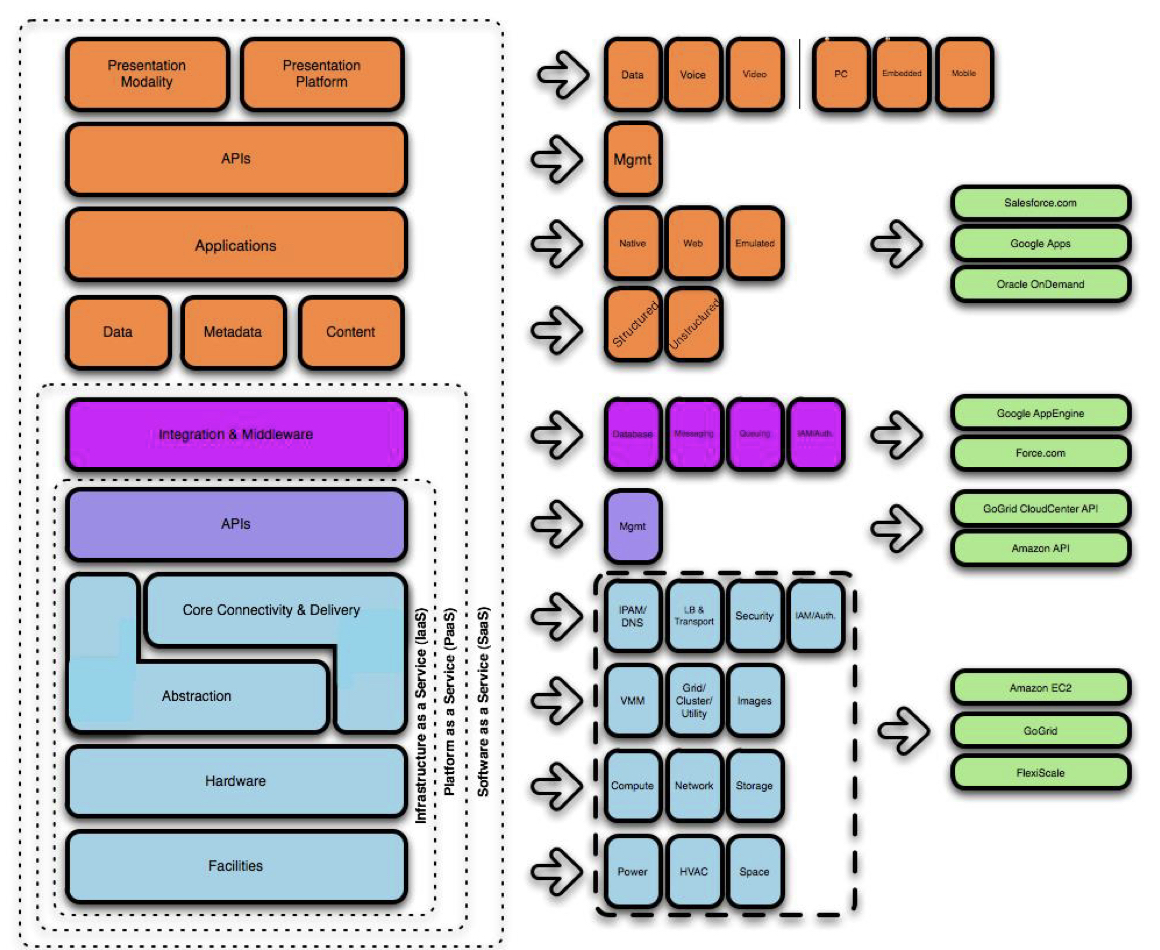
\includegraphics[scale=0.2]{img/cloud_stack.jpeg}
    \caption{The cloud stack, every layer of the XaaS stack is built on top of the services of the layer below}
\end{figure}
Cloud services can be deployed in a couple of different ways depending on who should have access to the services.

If the cloud infrastructure is provided exclusively for a single organization including multiple tenants is called private cloud, an example of private clud is the machine we can access via the cloud at SiLab in Unimi. The cloud infrastructure is owned and managed by a single organization (the solution can either be private or third party thus can be on premise or off premise).

If the cloud infrastructure is provided for an exclusive use of a community of users and is owned and managed by one or more organizations, thrd parties or a combination of the two we are talking about Community cloud.

If the cloud infrastructure is public we are talking about Public Cloud, an example of public cloud is OneDrive.

If the cloud infrastructure is a combination of two or more cloud infrastructures we are talking about Hybrid Cloud, each infrastructure remains separated, but are composed using standard or proprietary technologies.
